\chapter{Introduction and Motivation}\label{ch:intro}

Lung cancer is the most common cancer in the world in men, both in amount of cases and mortality. In women, is third in cases and second in mortality, after breast cancer\cite{WCR2014}. Yearly deaths due to lung cancer go over 1.5 million (see figure \ref{fig:world} for incidence), having around 10\% of five year survival rate in developed countries, and much lower in developing countries\cite{CRUK2014}. One over fourteen people has a lifetime risk of developing lung cancer\cite{Harrisons2012}, in average between men and women. The high incidence and mortality rates has lead to a big amount of research in research fields from all disciplines, in order to push further the detection and treatment of the disease, with an output of over 23.000 lung cancer related research articles in prestigious journals in the last 10 years\cite{Nature2015}. In addition, the  actual lung cancer treatment has been transformed from non-existent in the 70s to used worldwide\cite{Comis2003}.


\begin{figure}[ht]
\begin{center}
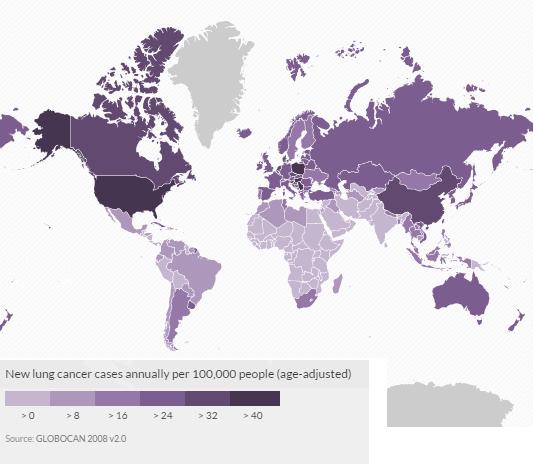
\includegraphics[width=0.98\columnwidth]{StateOfArt/worldmap.png}
\caption[Lung cancer incidence in the world]{Lung cancer incidence per country, age adjusted data. Map and data from {GLOBOCAN}\cite{GLOBOCAN2010}.}
%IARC has proprietary rights to the materials on the Website. Publications/data made available by IARC/WHO enjoy copyright protection in accordance with the provisions of Protocol 2 of the Universal Copyright Convention. All rights are reserved. Materials (fact sheets, maps, estimates or data) may be used "as is" for research, educational or other non-commercial purposes, but the corresponding reference must be cited in all cases.
\label{fig:world}
\end{center}
\end{figure}



The treatment of lung cancer varies between different types, but there are four main techniques: Chemotherapy, lobectomy or pneumoctomy, radiotherapy (RT) and palliative care. Generally, in early stages of small cell lung cancer the typical treatment would consist in chemotherapy with radiotherapy, and then brain radiotherapy, as there is chance that the tumour would spread to the head when treated. If the tumour has been detected in a very early stage and has not spread to the lymph nodes a lobectomy may be performed, removing part of the lung. Usually this is followed by radiotherapy and chemotherapy to make sure the tumour is killed.
In the case of non-small cell lung cancer, in the first stages a lobectomy or a pneumoctomy (removal of the whole lung) may be performed. Generally radiotherapy and chemotherapy (less likely) are also performed. In the last stages of the cancer, usually the treatment is palliative care i.e. treatments to reduce the symptoms and relief pain\cite{CRUK2014b}.

In practically all stages of different lung cancer treatments, radiotherapy is extensively used as above half of the treated patients do undergo the procedure\cite{Cancerorg}. About 120.000 patients use radiotherapy in the UK every year. Radiotherapy aims to kill malignant cells using ionizing radiation, generally using photons. High energy photons (X-rays) ionize the atoms that are part of the DNA chain. In photon therapy, this happens due to the ionization of the water in the cells, that forms free radicals, such as hydroxyl radicals, destroying the DNA of the cells and killing them.

Conventional photon RT is widely used around the world, nowadays generally guided by imaging systems during treatment planning (image guided radiation therapy, IGRT). Imaging systems, such as computed tomography (CT) and magnetic resonance imaging (MRI) are used to carefully tune the X-ray beam to focus in the specific location and shape of the tumour, and monitor the effects during the whole treatment period. However, a different type of radiation therapy exists, particle therapy or hardron therapy, that uses charged particles instead of photons, by accelerating them with circular particle accelerators. These particles (protons and heavy ions)  penetrate the tissue with minimal interaction and release almost all the energy before stopping. Figure \ref{fig:bragg} shows the energy deposition (dose) plotted versus the penetration of the energy beam in tissue. The energy burst that hardron show is refereed as the Bragg peak, after its discoverer William Henry Bragg. The Bragg peak allows for a radiation therapy where a larger amount of healthy tissue can be spared, while delivering highly spatially accurate doses to only the tumour areas. While the growth of hardron therapy has been slow in the past due to its cost, it is not being accelerated thanks to international collaboration projects such as ENLIGHT\cite{dosanjhparticle}, with 100 centres estimated by 2020 around the globe, 30 of them in Europe, 3 of them being already on their final stages in construction in the UK.

\begin{figure}[ht]
\begin{center}
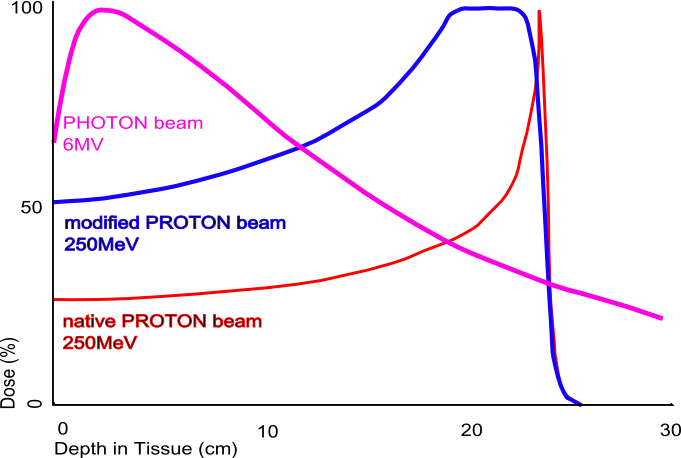
\includegraphics[width=0.6\columnwidth]{Introduction/BraggPeak.png}
\caption[Bragg peak]{The dose produced by a native and by a modified proton beam in passing through tissue, compared to the absorption of a photon or x-ray beam. From Wikimedia\cite{bragg}}
%GNU license, wikipedia
\label{fig:bragg}
\end{center}
\end{figure}


As previously mentioned, for both types of RT but specially for hadron therapy, imaging is generally used and needed for accurate treatment. Tumours not only are very different between patients, but also change considerably during treatment, so the patient does due to the physical toll of cancer treatment. This means that the tumour does change both shape and location, and that if these changes are not known, healthy tissue could be damaged and cancerous tissue spared. Generally patients will be imaged before each treatment, being one of the most common systems for imaging cone beam compute tomography (CBCT). CBCT takes few hundreds of seconds to scan a patient due to mechanical safety limitations. As one can foresee, this is an important limiting factor for tumours that move, such the liver and the lung ones, as the motion during acquisition can generate heave artefacts around the moving parts in image reconstruction. This moving effect is also a key factor to take into account in hadron therapy, as having a moving tumour means the high chance of missing the treatment target. Providing accurate imaging not only in space, but in time (4D imaging) is a key factor on treatment planning, an thus in cancer treatment. 

Interestingly, a motion compensation method for when objects are moving during adquisition was proposed by Hancock \textit{et al}\cite{pst1}\cite{pst2}\cite{pstweb} for monitoring the phase space of high energy particle bunches in particle accelerators at CERN. Phase space tomography is a hybrid algorithm that combines particle tracking in a computer model of a synchrotron with iterative reconstruction algorithms to reconstruct an image of the population of a bunch of particles circulating in the accelerator. The particle motion involves non-linear rotation and is non-cyclic, but a 1D projection of the distribution can be completely acquired as a single snapshot on one turn of the machine. By tracking test particles to gain a knowledge of how the geometry of the 2D image plane (longitudinal phase space) deforms, the information in all the discrete time slices acquired over many turns can be translated back to the same instant and tomographically combined in a single image.  Exploring the feasibility of using this tomographic motion compensation technique in medical applications is the objective of this thesis.


%% BLURRED IMAGE OF TUMOUR

\section{Aim of the thesis}

The CBCT and computed tomography (CT) in general image reconstruction problem is a complex mathematical and computational challenge, even for just 3D spatial reconstruction, without the additional problem of motion. Mathematically CT reconstruction is an ill-posed problem, as the solution may not be unique (as in circular CBCT) and generally the volume to reconstruct is considerably larger than the  data obtained, making the problem underdetermined. Often, an analytic approximated solution for the  mathematical problem is used, however this solution is considerably sensitive to noise and low amounts of data. As opposed to the analytic approximated solution, algebraic equation solving methods can be used. These generally lead to more robust solutions, especially in noisy an undersampled data. However, they require increased computational times, making them harder to introduce to clinical applications.

There are two main research problems tackled in this work:
\begin{itemize}
\item Firstly, this thesis explores the image reconstruction problem, in with focus on implementing accurate iterative algorithms, and accelerating them as much as possible, using GPU technology. The results from this part of the thesis are applicable to any CT application, from the medical one, to industrial or research cases. The work here explores a variety of algorithms for CT reconstruction, with both mathematical and computational focus.
\item Secondly, the thesis focuses in translating the motion compensation methods to the medical CBCT, focusing on IGRT applications, focusing also in the computational side of the method, as well as its robustness.
\end{itemize}

All the research presented here has been made public as part of the TIGRE Toolbox\cite{TIGRE} and can be found in a GitHub repository\cite{TIGREweb} for both MATLAB and Python. 

\section{Thesis organization}

The following chapters of the thesis are organized as following:

\subsubsection{Chapter 2: Image Guided Radiation Therapy and Computed Tomography}
\subsubsection{Chapter 3: The Image Reconstruction Problem}
\subsubsection{Chapter 4: GPU methods in tomography}
\subsubsection{Chapter 5: motion compensation modelling}
\subsubsection{Chapter 7: Numerical Study of Motion Compensation}
\subsubsection{Chapter 8: Discussion and conclusions}

\section{Publications and contributions}

The work on this thesis was been published either by open source software or publications in conferences and peer reviewed journals. The following publications directly relate to the content of this thesis:

\begin{itemize}
\item ``GPU based iterative CBCT for prospective motion compensated algorithm for radiation therapy''\cite{biguri2016gpu} . Short paper based on the presentation on the conference ICTR-PSE 2016.
\item ``TIGRE: A MATLAB-GPU toolbox for CBCT image reconstruction''\cite{TIGRE}. Journal article condensing the research in Chapter 3, Chapter 4 and Chapter 5.
\item  ``A General Method for Motion Compensation in X-ray Computed Tomography''\cite{biguri2017general}. Journal article on Chapter 6.
\end{itemize}

This work has been also presented in various conferences and meetings, via posters or presentations talks. Posters have been presented in ToScA 2016 with the title ``TIGRE: Tomographic Iterative GPU-based Reconstruction toolbox''\cite{biguri_ander_2016_159016}, in the ENLIGHT 2016 meeting titled ``Motion correction in X-ray tomography using a priori known deformation vector fields and iterative reconstruction methods''\cite{biguri2016motion} and in BIGART 2017 titled ``Improvement of image quality in 4D-CBCT respiratory correlated and motion-compensated reconstruction using iterative algorithms and GPU acceleration''\cite{biguri2017motion}. The work has also been presented in various talks and seminars. Finally, a Medical Physics Web article by Tami Freeman is available for wider audiences at \href{http://medicalphysicsweb.org/cws/article/research/66343}{http://medicalphysicsweb.org/cws/article/research/66343}.

The TIGRE Toolbox and specifically some of the total variation based image recosntruction code has been also used in the article ``Parameter selection in limited data cone-beam CT reconstruction using edge-preserving total variation algorithms'' by Lovithee \textit{et al}\cite{Vee}.

\subsubsection{Other publications}

During the length of the PhD, mainly in the early stages, other work was published mainly focused in dual modality electrical impedance tomography (EIT) - CBCT, as some initial work explored the use of EIT for real time tumour tracking. This work is not presented in this thesis, but has been published in few items. The work is summarized in a peer reviewed journal article ``Tracking boundary movement and exterior shape modelling in lung EIT imaging''\cite{biguri2015tracking}, and extended in peer-reviewed conference articles for the EIT 2015 meeting in the works titled ``Statistical and deterministic approaches for electrode movement in lung EIT''\cite{biguri2015statistical} and ``4D FEM models of the human thorax''\cite{biguri20154d}. Initial work on this field was also presented as a poster in the ENLIGHT 2014 meeting titled ``Dual modality EIT-CBCT for lung radiation therapy''\cite{biguri2015dual} and in AIP 2015 as ``Electrode movement due to breathing in lung EIT imaging''\cite{biguri2015electrode}.





